\documentclass[10.5pt,a4paper]{article}
\usepackage[a4paper,margin=2.2cm,top=2.3cm,bottom=2.4cm]{geometry}
\usepackage{fontspec}
\usepackage{unicode-math}
\setmainfont{TeX Gyre Pagella}
\setsansfont{Inter}[Scale=0.88]
\setmonofont{DejaVu Sans Mono}[Scale=0.80]
\setmathfont{DejaVu Math TeX Gyre}[Scale=0.95]
\usepackage{microtype}
\usepackage{xcolor}
\definecolor{accent}{HTML}{1F4E79}
\definecolor{muted}{HTML}{5F6670}
\definecolor{codebg}{HTML}{F6F7F9}
\definecolor{rule}{HTML}{D9DCE1}
\usepackage{graphicx}
\usepackage{booktabs,tabularx,array}
\usepackage{enumitem}
\setlist{nosep,leftmargin=1.4em,topsep=3pt}
\usepackage[font=small,labelfont={bf,sf},labelsep=period,skip=4pt]{caption}
\usepackage{titlesec}
\titleformat{\section}{\sffamily\large\bfseries\color{accent}}{\thesection}{0.7em}{}
\titleformat{\subsection}{\sffamily\normalsize\bfseries}{\thesubsection}{0.6em}{}
\titleformat{\subsubsection}[runin]{\sffamily\small\bfseries}{}{0em}{}[.]
\titlespacing*{\section}{0pt}{14pt}{6pt}
\titlespacing*{\subsection}{0pt}{10pt}{4pt}
\usepackage{fancyhdr}
\pagestyle{fancy}\fancyhf{}
\renewcommand{\headrulewidth}{0.4pt}
\renewcommand{\headrule}{\hbox to\headwidth{\color{rule}\leaders\hrule height \headrulewidth\hfill}}
\fancyhead[L]{\sffamily\footnotesize\color{muted}\ReportShortTitle}
\fancyhead[R]{\sffamily\footnotesize\color{muted}S. K. Eshraghi Naeini}
\fancyfoot[C]{\sffamily\footnotesize\color{muted}\thepage}
\usepackage{listings}
\lstdefinelanguage{VerilogX}[]{Verilog}{morekeywords={localparam,integer,genvar,generate,endgenerate}}
\lstset{language=VerilogX,basicstyle=\ttfamily\footnotesize,keywordstyle=\color{accent}\bfseries,
  commentstyle=\color{muted}\itshape,stringstyle=\color{teal!70!black},numbers=left,numberstyle=\tiny\color{muted},
  numbersep=6pt,backgroundcolor=\color{codebg},frame=single,rulecolor=\color{rule},framesep=4pt,
  xleftmargin=14pt,breaklines=true,columns=fullflexible,keepspaces=true,showstringspaces=false,
  tabsize=4,aboveskip=6pt,belowskip=6pt}
\usepackage{tikz}
\usetikzlibrary{arrows.meta,positioning,shapes.geometric,calc,fit,automata}
\tikzset{blk/.style={draw=accent,thick,fill=accent!6,rounded corners=2pt,minimum height=8mm,minimum width=20mm,align=center,font=\sffamily\small},
         io/.style={font=\sffamily\footnotesize,align=center},
         arr/.style={-{Stealth[length=2mm]},semithick},
         st/.style={state,draw=accent,thick,fill=accent!6,minimum size=9mm,font=\sffamily\footnotesize,inner sep=1pt,align=center}}
\usepackage{xurl}
\usepackage[colorlinks=true,linkcolor=accent,urlcolor=accent,citecolor=accent]{hyperref}
\usepackage{siunitx}
\sisetup{group-separator={,},group-minimum-digits=4}
\newcommand{\sig}[1]{\texttt{#1}}
\newcommand{\pass}{\textcolor{green!45!black}{\textsf{\textbf{PASS}}}}
\newcommand{\repo}{https://github.com/seyedkiarash/seyedkiarash.github.io/tree/main/labs/logic-circuits-lab}
\newcommand{\note}[1]{\par\smallskip\noindent\colorbox{accent!7}{\parbox{\dimexpr\linewidth-2\fboxsep}{\small #1}}\par\smallskip}
\setlength{\parindent}{0pt}
\setlength{\parskip}{4pt}

\newcommand{\ReportTitle}[3]{%
  \thispagestyle{plain}
  {\sffamily\small\color{muted}Logic Circuits Laboratory \textbullet\ Department of Electrical Engineering, Sharif University of Technology\par}
  \vspace{2pt}
  {\sffamily\LARGE\bfseries #1\par}
  \vspace{1pt}
  {\sffamily\Large #2\par}
  \vspace{6pt}
  {\color{rule}\hrule height 0.6pt}
  \vspace{5pt}
  {\small
  \begin{tabular}{@{}l@{\hspace{2em}}l@{}}
    \textcolor{muted}{Student}  & Seyed Kiarash Eshraghi Naeini (403101383)\\
    \textcolor{muted}{Instructor} & Dr.\ Mohammad Reza Movahhedin \quad\textcolor{muted}{Teaching assistant:} Hossein Moghim\\
    \textcolor{muted}{Semester} & Fall 2025 \quad\textcolor{muted}{session:} #3\\
    \textcolor{muted}{Platform} & Zynq-7010 (XC7Z010-CLG400-1), \SI{50}{MHz} clock, Vivado 2019.1
  \end{tabular}\par}
  \vspace{4pt}
  {\color{rule}\hrule height 0.6pt}
  \vspace{8pt}}

\newcommand{\ReportShortTitle}{Experiment 7 -- Seven-segment multiplexing and a stopwatch}
\begin{document}
\ReportTitle{7}{Seven-Segment Display Multiplexing, Counters and a Stopwatch}{27--29 December 2025}

\section*{Summary}
This experiment drives the four-digit seven-segment display of the lab board. Starting from a static
hexadecimal display, it introduces clock division, time-multiplexing of the digits, a scrolling text
display and finally a stopwatch built from cascaded modulo counters (\SI{0.1}{s} resolution, up to
9\,min\,59.9\,s). Three bonus designs extend the stopwatch with speed control and start/stop/reset buttons
and animate a ``snake'' around the display. Every design was re-verified for this report with a
self-checking Icarus Verilog testbench (9/9 pass) and re-synthesised with Yosys; the Vivado
implementation reports of the lab session show all timing constraints met. Two display errors found
during verification (Parts 2 and 5) are documented and corrected in Section~\ref{sec:changes}.
Source code, testbenches and constraint files: \url{\repo/lab07-seven-segment}.

\section{Hardware and conventions}
\begin{itemize}
  \item \textbf{Clock.} A \SI{50}{MHz} oscillator on pin U18 (\sig{create\_clock -period 20}).
  \item \textbf{Display.} Four digits share the seven segment lines \sig{a}--\sig{g}; \sig{dig[3:0]}
        selects the digits, \sig{dig[3]} being the leftmost. The segments are \emph{active-low}
        (a 0 lights a segment), the digit enables \emph{active-high}.
  \item \textbf{Decoder.} \sig{Hex\_to\_7\_seg} maps a 4-bit value to the segment pattern of
        \texttt{0}--\texttt{9}, \texttt{A}, \texttt{b}, \texttt{C}, \texttt{d}, \texttt{E}, \texttt{F}.
  \item \textbf{Clock divider.} A counter toggles its output every $H$ input cycles, so
        $f_\text{out} = f_\text{clk}/(2H)$. The values used in this experiment are listed in Table~\ref{tab:div}.
\end{itemize}

\begin{table}[h]
\centering\small
\caption{Clock divider settings ($f_\text{clk} = \SI{50}{MHz}$).}\label{tab:div}
\begin{tabular}{@{}lrrl@{}}
\toprule
Use & Half-period $H$ (cycles) & $f_\text{out}$ & Period \\
\midrule
Digit scanning (Parts 3, 5, 6, bonuses) & \num{12500} & \SI{2}{kHz} & \SI{0.5}{ms} per digit\\
Stopwatch tick (Part 6) & \num{2500000} & \SI{10}{Hz} & \SI{0.1}{s}\\
Stopwatch tick (Bonus A initial, Bonus B) & \num{5000000} & \SI{5}{Hz} & \SI{0.2}{s}\\
Student-number step (Part 2) & \num{12500000} & \SI{2}{Hz} & \SI{0.5}{s}\\
Moving digit / scrolling (Parts 4, 5) & \num{50000000} & \SI{0.5}{Hz} & \SI{2}{s}\\
\bottomrule
\end{tabular}
\end{table}

\section{Part 1 -- Static hexadecimal display}
\sig{DIP[3:0]} is decoded and all four digit enables are driven high. Because the digits share the
segment lines, every digit shows the same character (Fig.~\ref{fig:p1}). The testbench applies all 256
DIP settings and compares the segments with an independent reference table: 0 errors.
\begin{figure}[h]
\centering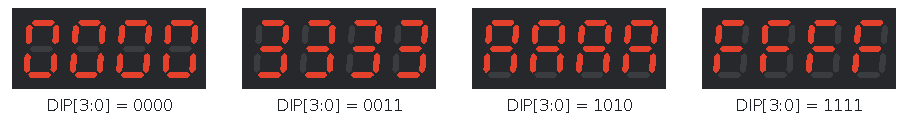
\includegraphics[width=0.78\linewidth]{figures/lab07_part1.pdf}
\caption{Part 1: with all digits enabled the same character appears four times.}\label{fig:p1}
\end{figure}

\section{Part 2 -- Student number, one digit at a time}
A \SI{2}{Hz} clock advances a state counter (0--9); a case statement maps each state to one digit of
the student number 403101383, shown on all four digits. State 9 shows \texttt{0} and acts as a short
pause before the sequence repeats. The testbench (step divider shortened to 4 cycles) records the
displayed sequence \texttt{4031013830}, as expected.

\section{Part 3 -- Time-multiplexing}
To show different characters on the four digits with only one set of segment lines, the digits are
enabled one at a time and the segment lines carry the character of the active digit. A \SI{2}{kHz}
scan clock steps a 2-bit counter; each digit is lit for \SI{0.5}{ms} and refreshed every
\SI{2}{ms} (\SI{500}{Hz}), far above the $\approx$\SI{60}{Hz} at which flicker becomes visible, so the
eye sees a steady \texttt{1234} (Fig.~\ref{fig:p3}). Multiplexing needs $7+4=11$ outputs instead of
$4\times7=28$.
\begin{figure}[h]
\centering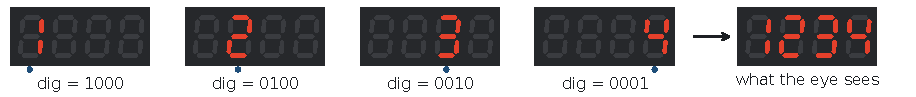
\includegraphics[width=\linewidth]{figures/lab07_part3_frames.pdf}\\[4pt]
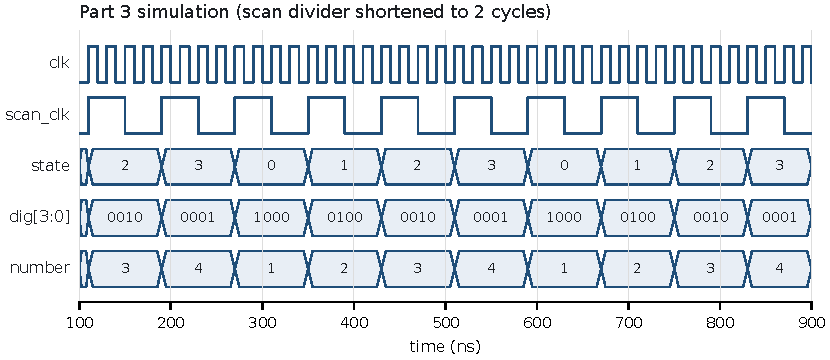
\includegraphics[width=0.9\linewidth]{figures/lab07_part3_wave.pdf}
\caption{Part 3: the four scan states and the perceived image (top); simulation with the scan divider
shortened to 2 cycles (bottom) -- \sig{dig} rotates \texttt{1000}$\to$\texttt{0100}$\to$\texttt{0010}$\to$\texttt{0001}
together with the digit value.}\label{fig:p3}
\end{figure}

The testbench reconstructs the image from the enable and segment signals and checks that exactly one
digit is enabled at any time: frame \texttt{"1234"}, 0 one-hot violations.

\section{Part 4 -- A moving digit}
The same rotating enable as in Part 3, but driven by a \SI{0.5}{Hz} clock and with a constant value: the
digit \texttt{3} jumps one position to the right every \SI{2}{s}. Running the rotation slowly makes the
mechanism of Part 3 visible. The testbench checks that the character is always \texttt{3} and that each
move goes exactly one position to the right (25 moves, 0 errors).

\section{Part 5 -- Scrolling student number}
Two clocks are derived from the board clock: the \SI{2}{kHz} scan clock of Part 3 and a \SI{0.5}{Hz}
shift clock that selects one of nine 4-digit windows over the student number (with wrap-around), so the
number scrolls across the display (Fig.~\ref{fig:p5}). The window is held in a 16-bit register
\sig{numbers\_state} whose top nibble is the first (leftmost) digit.
\begin{figure}[h]
\centering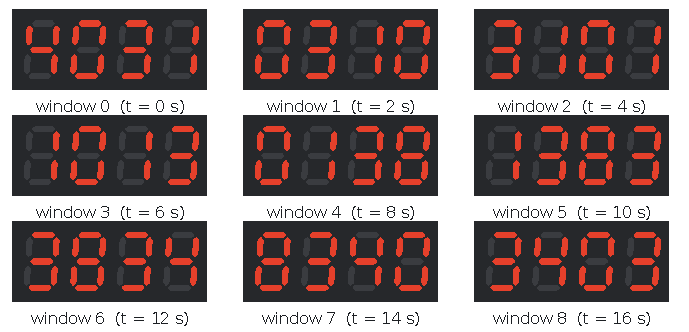
\includegraphics[width=0.62\linewidth]{figures/lab07_part5.pdf}
\caption{Part 5: the nine windows shown by the corrected design, one every \SI{2}{s}.}\label{fig:p5}
\end{figure}

The testbench shortens both dividers, reconstructs the full display image in every window and compares
it with the expected text: 9/9 windows correct.

\section{Part 6 -- Stopwatch}
\subsection{Design}
Four modulo counters form the time \texttt{M SS.d}: tenths (mod 10), seconds (mod 10), tens of seconds
(mod 6) and minutes (mod 10). All counters share the \SI{10}{Hz} tick clock and are cascaded
\emph{synchronously}: each counter is enabled by the \sig{done} output of the previous one, which is
asserted while that counter is enabled and at its terminal count. The digits are multiplexed as in
Part 3 with the tenths on the rightmost digit (Fig.~\ref{fig:sw}).

\begin{figure}[h]
\centering
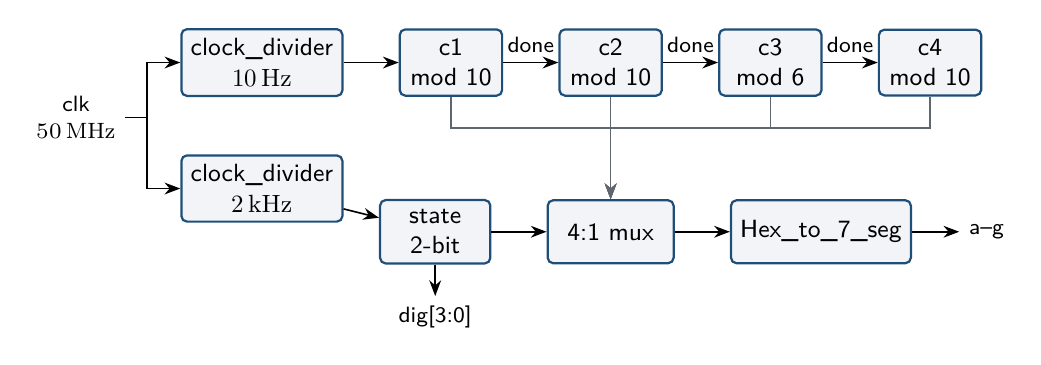
\begin{tikzpicture}[node distance=5mm and 7mm]
  \node[io] (clk) {clk\\\SI{50}{MHz}};
  \node[blk,right=of clk,yshift=7mm] (tick) {clock\_divider\\\SI{10}{Hz}};
  \node[blk,right=of clk,yshift=-9mm] (scan) {clock\_divider\\\SI{2}{kHz}};
  \node[blk,right=of tick,minimum width=13mm] (c1) {c1\\mod 10};
  \node[blk,right=of c1,minimum width=13mm] (c2) {c2\\mod 10};
  \node[blk,right=of c2,minimum width=13mm] (c3) {c3\\mod 6};
  \node[blk,right=of c3,minimum width=13mm] (c4) {c4\\mod 10};
  \node[blk,below=13mm of c2,minimum width=16mm] (mux) {4:1 mux};
  \node[blk,right=of mux] (dec) {Hex\_to\_7\_seg};
  \node[io,right=6mm of dec] (seg) {a--g};
  \node[blk,left=of mux,minimum width=14mm] (st) {state\\2-bit};
  \node[io,below=4mm of st] (dig) {dig[3:0]};
  \draw[arr] (clk) -- ++(9mm,0) |- (tick);
  \draw[arr] (clk) -- ++(9mm,0) |- (scan);
  \draw[arr] (tick) -- (c1);
  \draw[arr] (c1) -- node[above,io]{done} (c2);
  \draw[arr] (c2) -- node[above,io]{done} (c3);
  \draw[arr] (c3) -- node[above,io]{done} (c4);
  \draw[arr] (scan) -- (st);
  \draw[arr] (st) -- (mux);
  \draw[arr] (st) -- (dig);
  \foreach \c in {c1,c2,c3,c4} \draw[arr,muted] (\c.south) -- ++(0,-4mm) -| (mux.north);
  \draw[arr] (mux) -- (dec);
  \draw[arr] (dec) -- (seg);
\end{tikzpicture}
\caption{Stopwatch architecture. All counters are clocked by the \SI{10}{Hz} tick; the \sig{done}
signals act as synchronous carry/enable.}\label{fig:sw}
\end{figure}

\begin{lstlisting}[caption={Modulo counter with enable and carry (\texttt{mod\_counter.v}).}]
always @(posedge clk)
    if (enable)
        number <= (number == N) ? 4'd0 : number + 4'd1;

assign done = enable && (number == N);   // next counter advances on this tick
\end{lstlisting}

\subsection{Verification}
With the tick shortened to 32 clock cycles, the testbench runs the stopwatch through a complete cycle of
6000 ticks (including the roll-over \texttt{9:59.9}$\to$\texttt{0:00.0}) and after every tick reads the
multiplexed display and compares it with the elapsed time: 6003/6003 readings correct.
Fig.~\ref{fig:swwave} shows the carry chain.
\begin{figure}[h]
\centering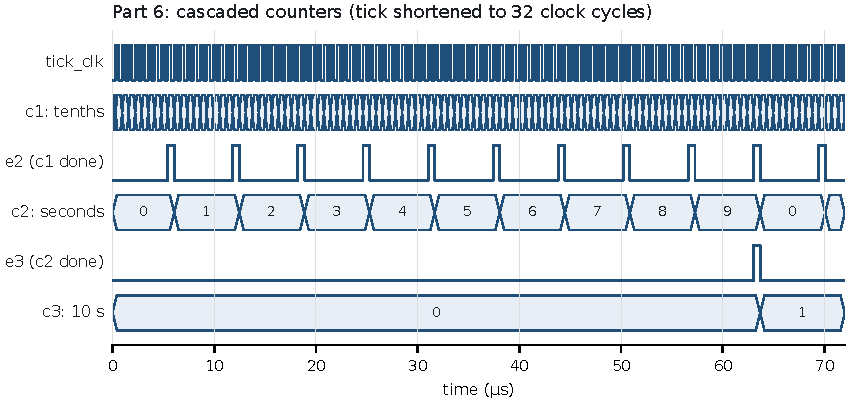
\includegraphics[width=0.9\linewidth]{figures/lab07_part6_wave.pdf}\\[4pt]
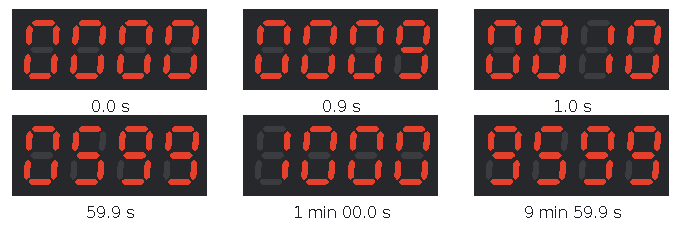
\includegraphics[width=0.62\linewidth]{figures/lab07_part6.pdf}
\caption{Part 6: c2 advances once per ten ticks (on \sig{e2}), c3 once per hundred (on \sig{e3});
bottom: display readings at selected times.}\label{fig:swwave}
\end{figure}

\section{Bonus tasks}
\subsection{A -- Adjustable speed}
The tick divider is replaced by a divider whose half-period is a register: a rising edge on
\sig{button[1]} doubles it (slower) and on \sig{button[2]} halves it (faster); edges are found by comparing
each button with its value one clock earlier. Simulated: tick period 16$\to$32 cycles after
\sig{button[1]}, then 8 after two presses of \sig{button[2]}.

\subsection{B -- Start, stop and reset}
\sig{button[1]} clears and \sig{button[2]} sets a \sig{run} flag that enables the first counter (the
stopwatch powers up stopped); \sig{button[3]} synchronously clears all counters. Simulated sequence:
power-up \texttt{0000}, counting after start, value held while stopped, \texttt{0000} after reset.

\subsection{C -- Snake}
The outer segments of the four digits form a ring of 12 positions (top row left to right, the right
side of digit 0, the bottom row right to left, the left side of digit 3). A 3-segment snake advances
one position per \SI{0.67}{s}: a combinational block ORs the masks of the head and the two
following positions into a pattern per digit, and the patterns are multiplexed at \SI{381}{Hz}. Timing
comes from taps of a free-running counter (bits 16 and 24). The testbench records one full loop and
checks that every frame has exactly three lit segments (Fig.~\ref{fig:snake}).
\begin{figure}[h]
\centering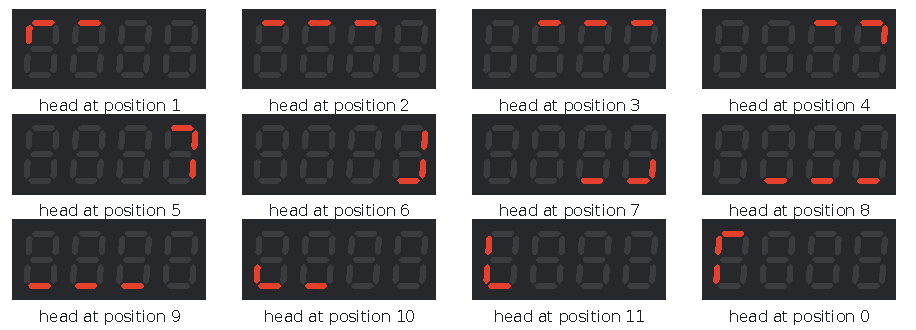
\includegraphics[width=0.82\linewidth]{figures/lab07_snake.pdf}
\caption{Bonus C: one loop of the snake reconstructed from the simulation.}\label{fig:snake}
\end{figure}
\note{In this design the digit enables are driven \emph{active-low} (\texttt{1110} selects digit 0),
whereas Parts 3--6 drive them active-high (\texttt{0001}). The cleaned version keeps the submitted
behaviour behind a parameter \sig{DIGIT\_ACTIVE\_LOW} (default 1); with the board's active-high enables it
should be set to 0.}

\section{Implementation results}
Table~\ref{tab:impl} is taken from the Vivado reports of the lab session (XC7Z010, 17\,600 LUTs,
35\,200 flip-flops). All designs meet the \SI{20}{ns} clock constraint with a large margin.
\begin{table}[h]
\centering\small
\caption{Vivado post-implementation results.}\label{tab:impl}
\begin{tabular}{@{}lrrrr@{}}
\toprule
Design & LUTs & Flip-flops & WNS (ns) & Timing \\
\midrule
Part 5 -- scrolling student number & 29 & 72 & 14.893 & met\\
Part 6 -- stopwatch & 42 & 84 & 15.393 & met\\
Bonus B -- stopwatch with start/stop/reset & 47 & 88 & 14.655 & met\\
Bonus C -- snake & 116 & 48 & 17.608 & met\\
\bottomrule
\end{tabular}
\end{table}

\textbf{Design note.} The divided clocks are used directly as clocks of other registers. This works at
these rates, but the static timing analysis only covers the \SI{50}{MHz} domain unless the generated
clocks are constrained. The usual alternative -- keeping one clock and using one-cycle \emph{enable}
pulses -- is the style used in the second ping-pong game of Experiment~6.

\section{Changes made during this review}\label{sec:changes}
\begin{itemize}
  \item \textbf{Part 2.} State 3 displayed \texttt{4} instead of \texttt{1}, so the sequence read
        4\,0\,3\,\textbf{4}\,0\,1\,3\,8\,3. Corrected.
  \item \textbf{Part 5.} The leftmost digit (\sig{dig = 1000}) was given the \emph{last} nibble of the window,
        so every window appeared mirrored (e.g.\ \texttt{0310} shown as \texttt{0130}, confirmed by
        simulating the submitted code). The nibble order of the scan multiplexer was reversed.
  \item \textbf{All parts.} Dividers became parameters (so testbenches can shorten them), registers
        received initial values, unused modules were removed, and comments were rewritten in English
        (the original Persian comments had been saved as \texttt{?} characters and were not recoverable).
\end{itemize}

\section{Verification summary}
\begin{table}[h]
\centering\small
\begin{tabularx}{\linewidth}{@{}lXr@{}}
\toprule
Testbench & What is checked & Result\\
\midrule
\sig{tb\_show4dig} & all 256 DIP settings against a reference decoder & \pass\\
\sig{tb\_show\_student\_id} & displayed digit sequence & \pass\\
\sig{tb\_display\_1234} & reconstructed image, one digit enabled at a time & \pass\\
\sig{tb\_moving\_digit} & character and direction of every move & \pass\\
\sig{tb\_scrolling\_student\_id} & image of all 9 windows & \pass\\
\sig{tb\_stopwatch} & display after each of 6003 ticks incl.\ roll-over & \pass\\
\sig{tb\_stopwatch\_speed\_control} & tick period after the speed buttons & \pass\\
\sig{tb\_stopwatch\_start\_stop} & power-up, start, stop (hold), reset & \pass\\
\sig{tb\_snake\_display} & one loop, three lit segments per frame & \pass\\
\bottomrule
\end{tabularx}
\end{table}
Reproduce with \texttt{scripts/run\_sims.sh lab07-seven-segment} (Icarus Verilog 12).

\section{Conclusion}
Time-multiplexing lets four digits be driven by eleven pins as long as each digit is refreshed well
above the flicker threshold; here a \SI{2}{kHz} scan gives a \SI{500}{Hz} refresh. Synchronous
cascading through \sig{done}/\sig{enable} turns simple modulo counters into a multi-digit stopwatch,
and the same structure accepts run control and speed control with a few registers. Simulating the
displayed image -- not just the internal signals -- was what exposed the two display-order errors.

\end{document}
